\section{Durchführung}
\label{sec:Durchführung}

\subsection{Versuchsaufbau}
\label{sec:Versuchsaufbau}
%\begin{figure}
%	\centering
%	\caption{Schematische Darstellung des Versuchsaufbaus \cite{anleitung}.}
%	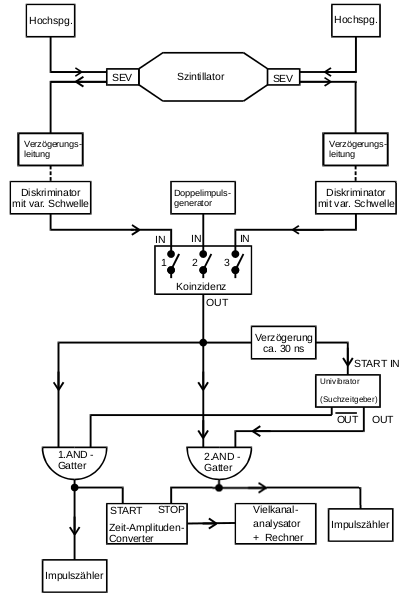
\includegraphics{Bilder/aufbau.png}
%	\label{fig:aufbau}
%\end{figure}
%
%\begin{figure}
%	\centering
%	\caption{Schematische Darstellung der Quelle zur Erzeugung radioaktiven Isotopen \cite{anleitung}.}
%	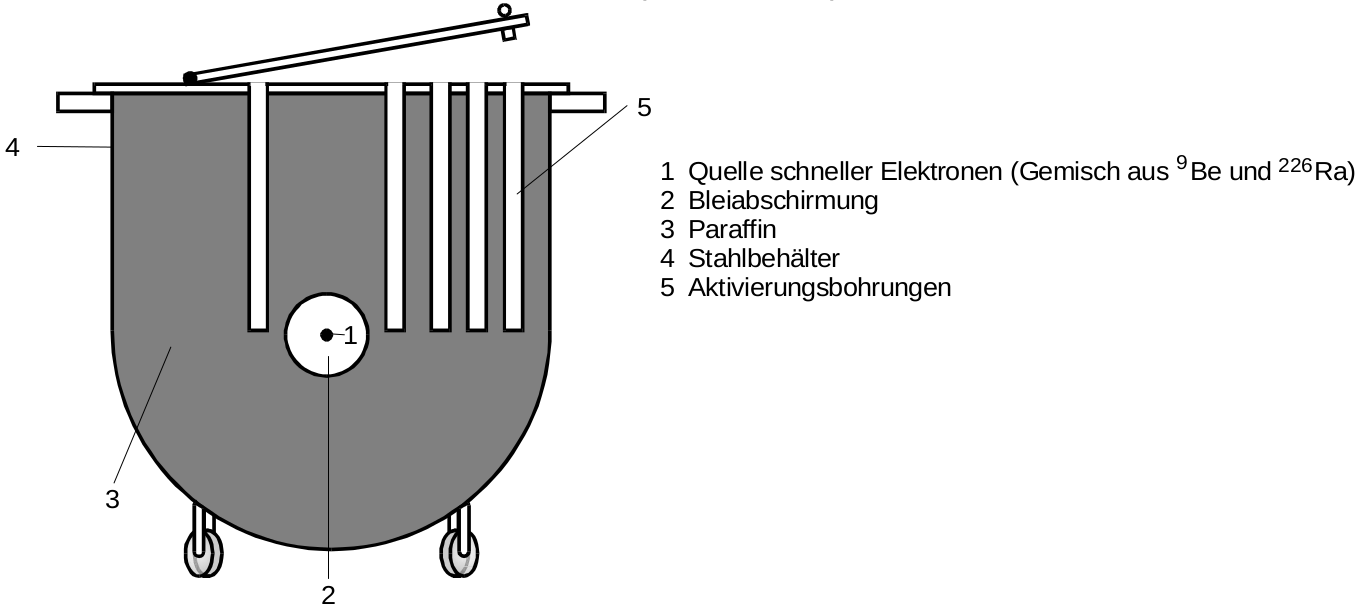
\includegraphics{content/toepfchen.png}
%	\label{fig:kochen}
%\end{figure}
%
Der Versuchsaufbau -- wie in Abbildung \ref{fig:aufbau} dargestellt -- besteht im Wesentlichen 
aus einem zerfallenden radioaktiven Isotop und einem Geiger-Müller-Zählrohr, welches die 
zerfallenden Kerne misst.
Das Geiger-Müller-Zählrohr ist entspricht einer mit Gas gefüllten Röhre. Trifft ein $\beta$-
oder $\gamma$- Teilchen auf ein Gasteilchen wird dieses ionisiert und kann aufgrund einer
anliegenden Spannung an der Röhre gemessen werden.
Dabei werden die gemessenen Zerfälle pro Messzeitintervall, welches am Zeitgeber einstellbar 
ist, an den Zählern 1 und 2 angezeigt. Nach jedem Messvorgang wird der Zähler umgeschaltet und 
der vorherige Wert auf dem aktuellen Zähler wird überschrieben. Der Versuchsaufbau ist mit
einer Blei-Abschirmung ausgestattet um die radioaktive Strahlung abzuschirmen.

Zur Erzeugung der radioaktiven Isotope wird das Objekt in Abbildung \ref{fig:kochen} verwendet.
Hierbei werden stabile Kerne mit niederenergetischen Neutronen beschossen. 
Da die Neutronen ihre Energie durch elastische Stöße an die Kerne übergeben und die maximale
Energie bei gleichen Massen der Stoßpartner erreicht wird, werden die Neutronen in einem 
Paraffinmantel gebremst, bis sie die optimale Energie besitzen.


\subsection{Versuchsbeschreibung}
\label{sec:Versuchsbeschreibung}
Zu Beginn der Messung werden die verwendeten Acrylzylinder ebenso wie die Acrylplatten mit einer Schiebelehre vermessen.
Über einen Drehschalter lässt sich das Messverfahren am Ultraschallechoskop einstellen.
Für das Impuls-Echo-Verfahren ist dieser Drehschalter auf die Position 1/1, bzw. 2/2 zu drehen, jenachdem mit welcher Sonde die Messung durchgeführt wird.\\
Für das Durchschallungsverfahren wird der Modus 1/2 bzw. 2/1 gewählt.
Eine Sonde ist hierbei jeweils der Sender und die andere Sonde dient als Empfänger.
Für die Messung der Laufzeit mit dem Impuls-Echo Verfahren wird eine Sonde über bidestilliertes Wasser an einen Acrylzylinder gekoppelt, welcher auf ein Papiertuch zu stellen ist, um Kratzer am Versuchsobjekt zu vermeiden.\\
In das Messprogramm ist zur Berechnung der Eindringtiefe die Schallgeschwindigkeit $c$ nach den Literaturdaten, bzw. die durch eine Laufzeitmessung nach Formel \eqref{eqn:laufzeit} ermittelte Schallgeschwindigkeit einzutragen.
Um Impulse eindeutiger identifizieren zu können, kann für Laufzeitmessungen die Amplitude über die Einstellung am Ultraschallechoskop verstärkt werden.\\
Die Messung mit dem Impuls-Echo-Verfahren zur Bestimmung der Schallgeschwindigkeit soll für sieben verschiedene Zylinderlängen erfolgen. Hierfür können auch mehrere Zylinder gestapelt werden
Mittels des Impuls-Echo-Verfahrens soll zudem die Dämpfungskonstante des Zylindermaterials bestimmt werden. Zu Beachten ist, dass hierfür keinesfalls eine Verstärkung verwendet werden darf. Außerdem dürfen keine Zylinder gestapelt werden, da sich an der Übergangsfläche sowohl eine reflektierte, als auch eine transmittierte Schallwelle bildet, somit ist eine Bestimmung des Amplitudenverhältnis nicht sinnvoll.
Es sollen möglichst viele Zylinderlängen vermessen werden. Für große Zylinderlängen kann allerdings die Amplitude der reflektierten Schallwelle so gering ausfallen, dass sie nicht mehr zu bestimmen ist.
\\Zudem soll die Schallgeschwindigkeit für möglichst viele Zylinder mit dem Durchschallverfahren bestimmt werden. Hierfür wird beidseitig an den Acrylzylinder, welcher in eine Halterung waagerecht gelegt wird, jeweils eine Sonde mit Kopplungsgel gekoppelt.
Zur Analyse eines Spektrums/Cepstrums wird ein etwa \SI{40}{\milli\meter} langer Acrylzylinder auf zwei Acrylplatten gesetzt sowie eine Sonde an den Zylinder gekoppelt.
Alle Grenzflächen werden durch bidestilliertes Wasser gekoppelt. Die Verstärkung ist so zu wählen, dass 3 Mehrfachreflexionen zu erkennen sind.
Im A-Scan werden die beiden Cursor so neben die Mehrfachreflexionen gesetzt, dass ein Spektrum/Cepstrum mittels der FFT-Funktion erzeugt werden kann.\\
Zur Untersuchung der Innenabstände des Augenmodells wird eine Messung mit dem Impuls-Echo-Verfahren durchgeführt. Hierzu wird eine Sonde mit Koppelgel vorsichtig auf die Hornhaut des Augenmodells gesetzt und vorsichtig so ausgerichtet, dass im Messprogramm fünf Peaks zu erkennen sind (Reflektion durch die Hornhaut, Iris, Vorder- und Rückseite der Linse und der Retina).
